\documentclass[a4paper,12pt]{article}
\usepackage{xltxtra}
\usepackage{fancyhdr}
\usepackage[top=1in, bottom=1.5in, left=1cm, right=1cm]{geometry}
\usepackage{setspace}
\usepackage{bbm}
\usepackage{algorithmicx}
\usepackage{algpseudocode}
\usepackage{algorithm}
\usepackage{graphicx}
\newcommand*\Let[2]{\State #1 $\gets$ #2}
\onehalfspacing
% Chestiile pentru mate
\usepackage{amsmath}
\usepackage{amsfonts}
\usepackage{bbm}
\author{Roland Szabo, gr. 235}
\usepackage{fancyhdr}
\pagestyle{fancy}
\makeatletter
\makeatother
\lhead{Roland Szabo, gr. 235}
\rhead{Lab 2, 06.11.13}
\begin{document}

\section{Problem statement}
Create a program than contains an implementation of 3 different algorithms for computing the greatest common divisor of 2 natural numbers.

Show a graph of the running time of these algorithms. 

\section{Algorithms}
\subsection{Prime factorization}
	\begin{algorithmic}
		\Ensure{$ b c = gcd(a,b) $}
		\Procedure{prime\_factorization}{a,b}
			\Comment{ Complexity: $ \theta (2^n) $ }
			\Let{$ div_a $}{divisors(a)}
			\Let{$ div_b $}{divisors(b)}
			\Let{$ div_c $}{ $ div_a \cap div_ b $}
			\Let{prime\_factorization}{$\prod div_c $}
		\EndProcedure	
	\end{algorithmic}

\subsection{Euclid's algorithm}
	\begin{algorithmic}
		\Ensure{$ b c = gcd(a,b) $}
		\Procedure{euclid}{a,b}
			\Comment{ Complexity: $ \theta (n) $ }
			\If{$ a == 0 $}
				\Let{euclid}{b}
			\EndIf
			\If{$ b == 0 $}
				\Let{euclid}{a}
			\EndIf
			\While{$ a > 0 $}
				\Let{temp}{a}
				\Let{a}{$ b \mod a $}
				\Let{b}{temp}				
			\EndWhile
			\Let{euclid}{a}
		\EndProcedure	
	\end{algorithmic}

\subsection{Stein}
	\begin{algorithmic}
		\Ensure{$ b c = gcd(a,b) $}
		\Procedure{euclid}{a,b}
			\Comment{ Complexity: $ \theta (n) $ }
			\If{$ b == a $}
				\Let{euclid}{a}
			\EndIf
			\If{$ a == 0 $}
				\Let{euclid}{b}
			\EndIf
			\If{$ b == 0 $}
				\Let{euclid}{a}
			\EndIf
			\If{$a \mod 2 = 0 $}
			    \If{$ b \mod 2 = 1 $}
	    			\Let{stein}{$ stein(a/2, b) $}
				\Else
					\Let{stein}{$ stein(a/2, b/2) * 2 $}
				\EndIf
			\EndIf
		    \If{$ b \mod 2 = 0 $}
    			\Let{stein}{$ stein(a, b/2) $}
    		\EndIf
    		\If{$a > b$}
    			\Let{stein}{$stein((u-v)/2, v)$}
    		\Else
	    		\Let{stein}{$stein((v-u)/2, u)$}
	    	\EndIf
		\EndProcedure	
	\end{algorithmic}

	
\section{Runtime analysis}

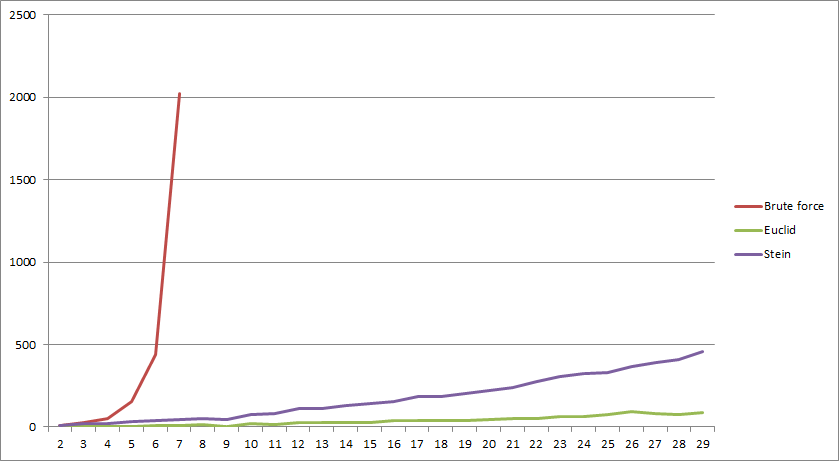
\includegraphics{graph.png}

As can be seen from the graph, the naive, brute-force algorithm has an exponential complexity, and can't be used with numbers with more than 7-8 digits. Stein's and Euclid's algorithms are linear in time, but Euclid's has a smaller overhead, because it doesn't involve doing so many comparisons and divisions. 

\end{document}